\pdfmapfile{+univers}%
\pdfmapfile{+dinbold}%
\documentclass[ngerman]{beamer}
\usepackage[utf8]{inputenc}
\usepackage[T1]{fontenc}
\usepackage[ngerman]{babel}
\usepackage{graphicx}
\usepackage{svg}
\usetheme[pagenum,nosectionnum,noheader,transition=push,headline=light]{tud}
\begin{document}
\title{FoodShip Group Update}
\subtitle{FoodShip, a foodsharing App}
\author{Sönke Huster \& Hannes Hilbert}
\date{\today}

\maketitle

  %  \frame{\frametitle{Inhaltsverzeichnis}\tableofcontents}

\section{Foodship}
\frame{\frametitle{Foodship App Scenario}
    \begin{itemize}
        \item App proposes having dinner with users nearby and a recipe based on the groups fridge content
    \end{itemize}
    \begin{figure}
        \begin{center}
            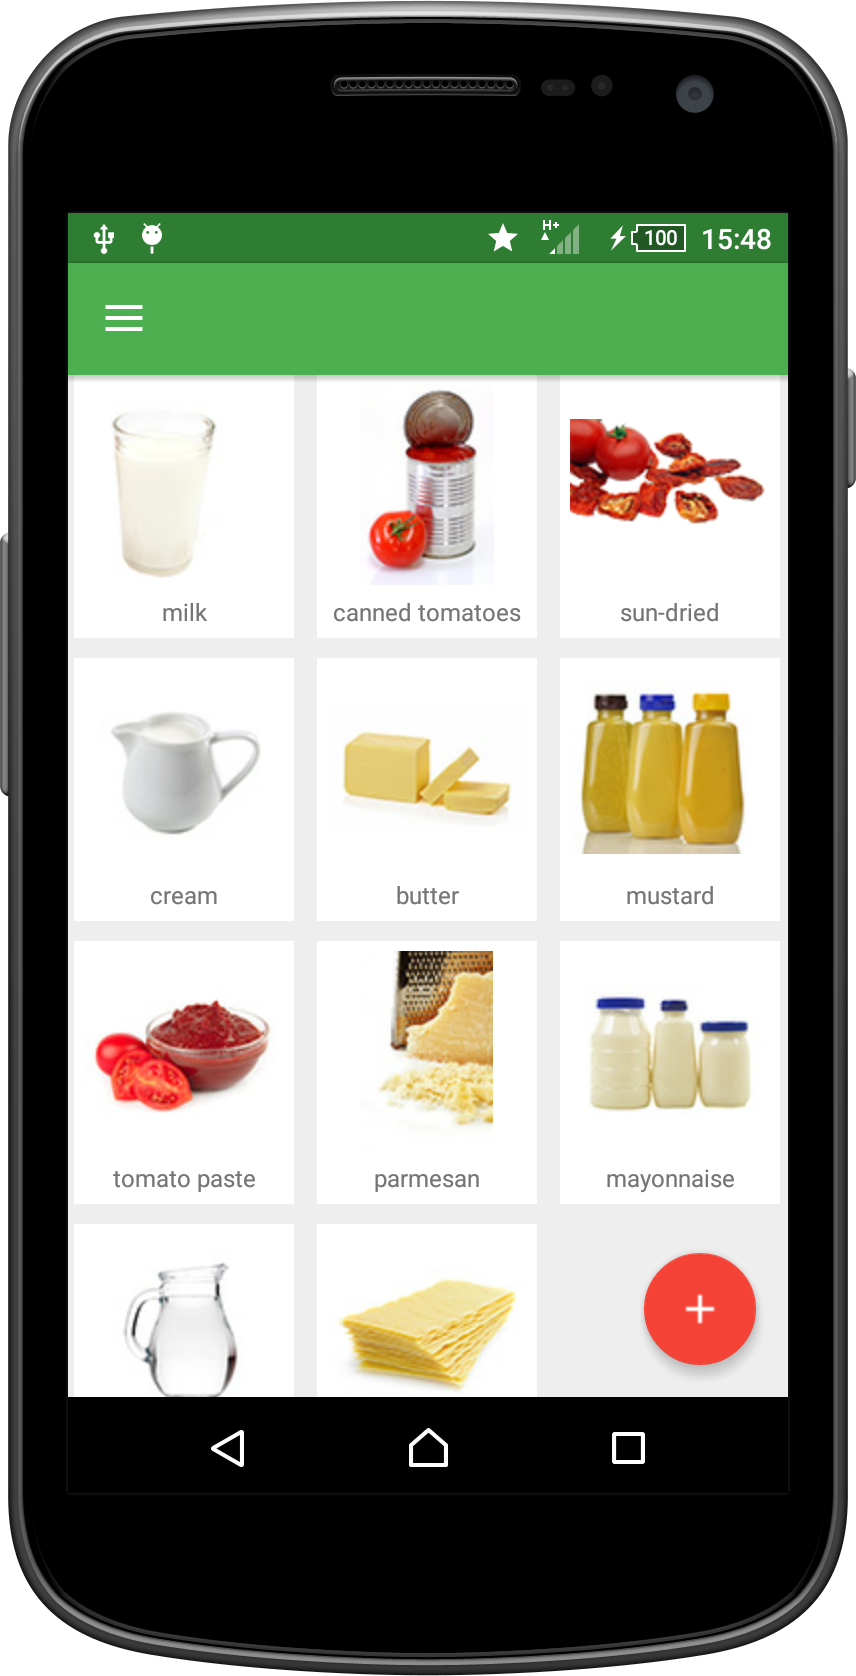
\includegraphics[width=0.25\textwidth,height=\textheight,keepaspectratio]{../screenshots/overview.png}
            \hspace{1cm}
            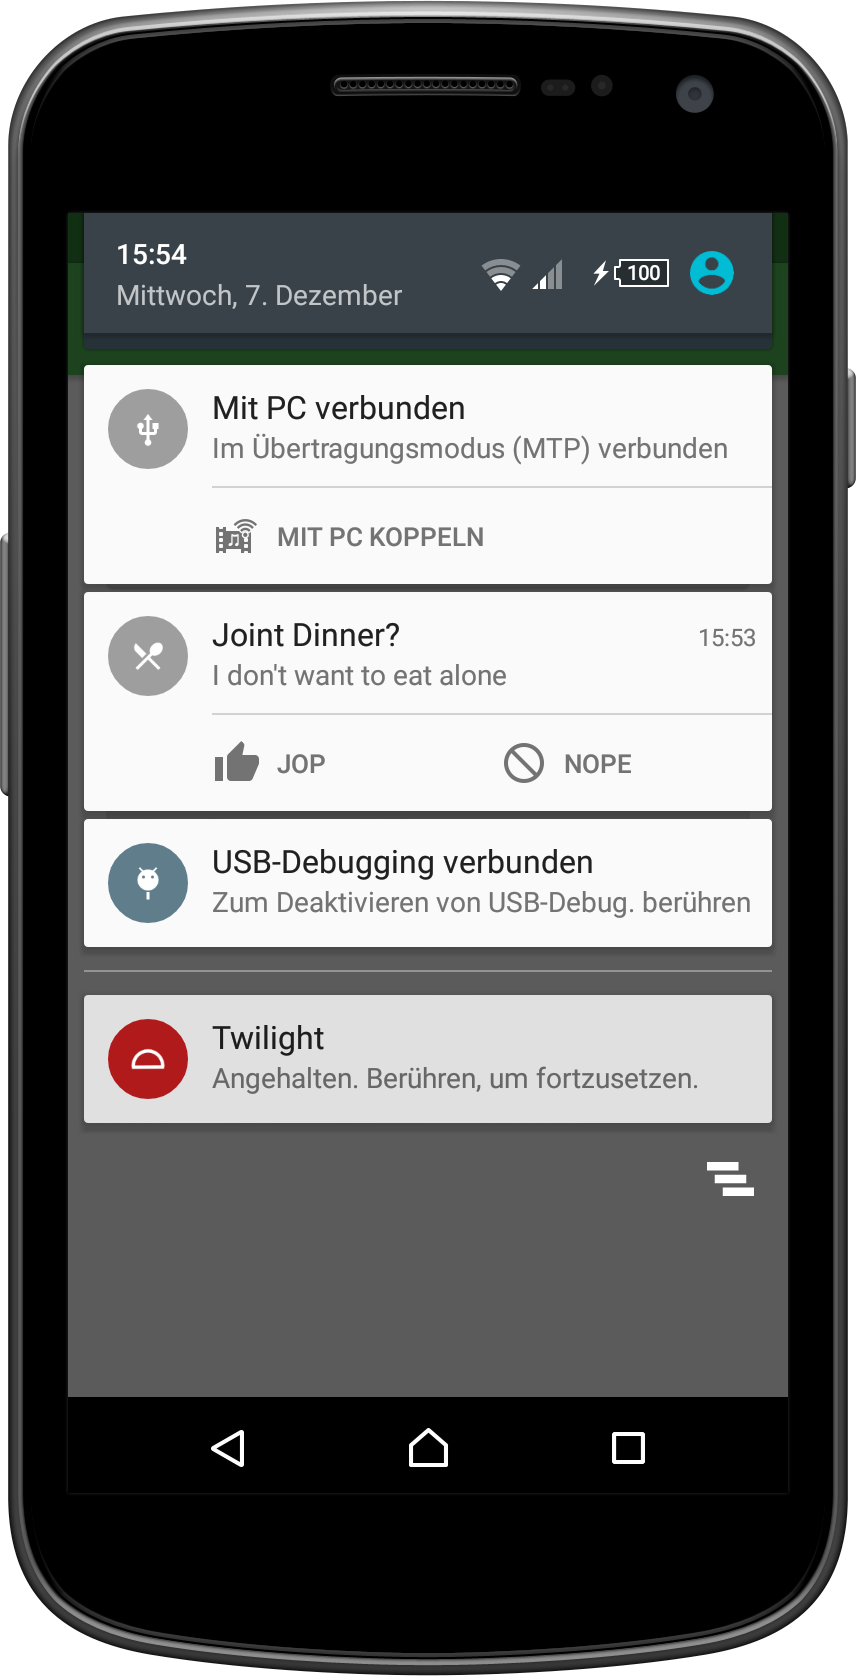
\includegraphics[width=0.25\textwidth,height=\textheight,keepaspectratio]{../screenshots/notification.png}
            \hspace{1cm}
            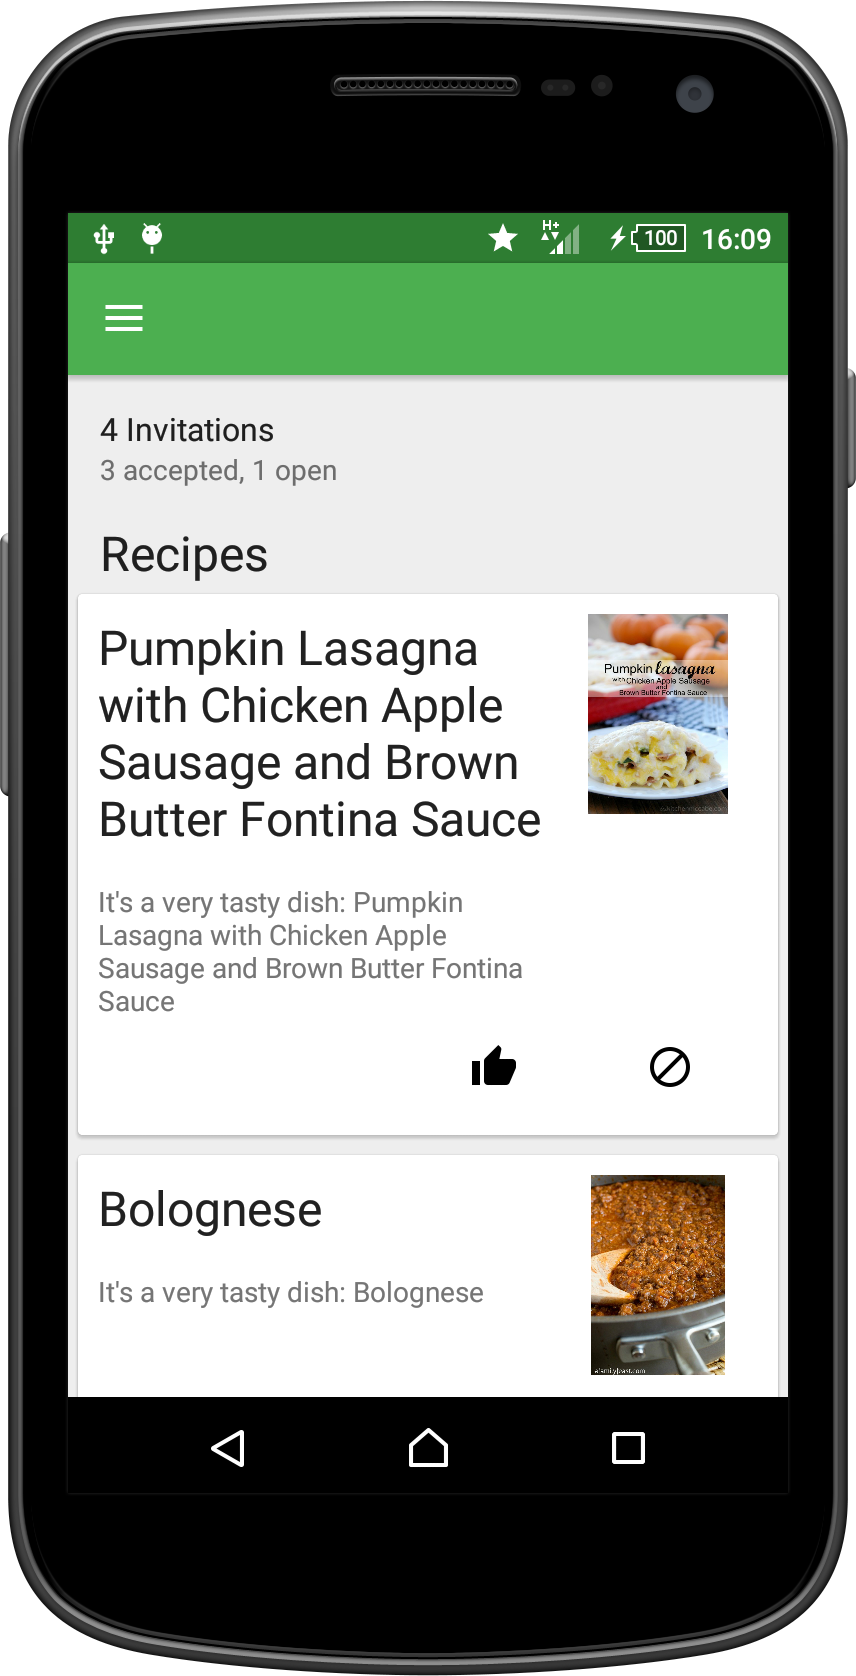
\includegraphics[width=0.25\textwidth,height=\textheight,keepaspectratio]{../screenshots/recipe_overview.png}
        \end{center}
    \end{figure}

}

\section{Adaptation on User Context}
    \frame{\frametitle{Ingredient adaptation}
        \begin{itemize}
            \item Suggest recipes that match many ingredients
            \item Example: Six of eleven ingredients needed for the best match
            \item Server regulary gets matching recipes
        \end{itemize}
        \begin{figure}
            \begin{center}
                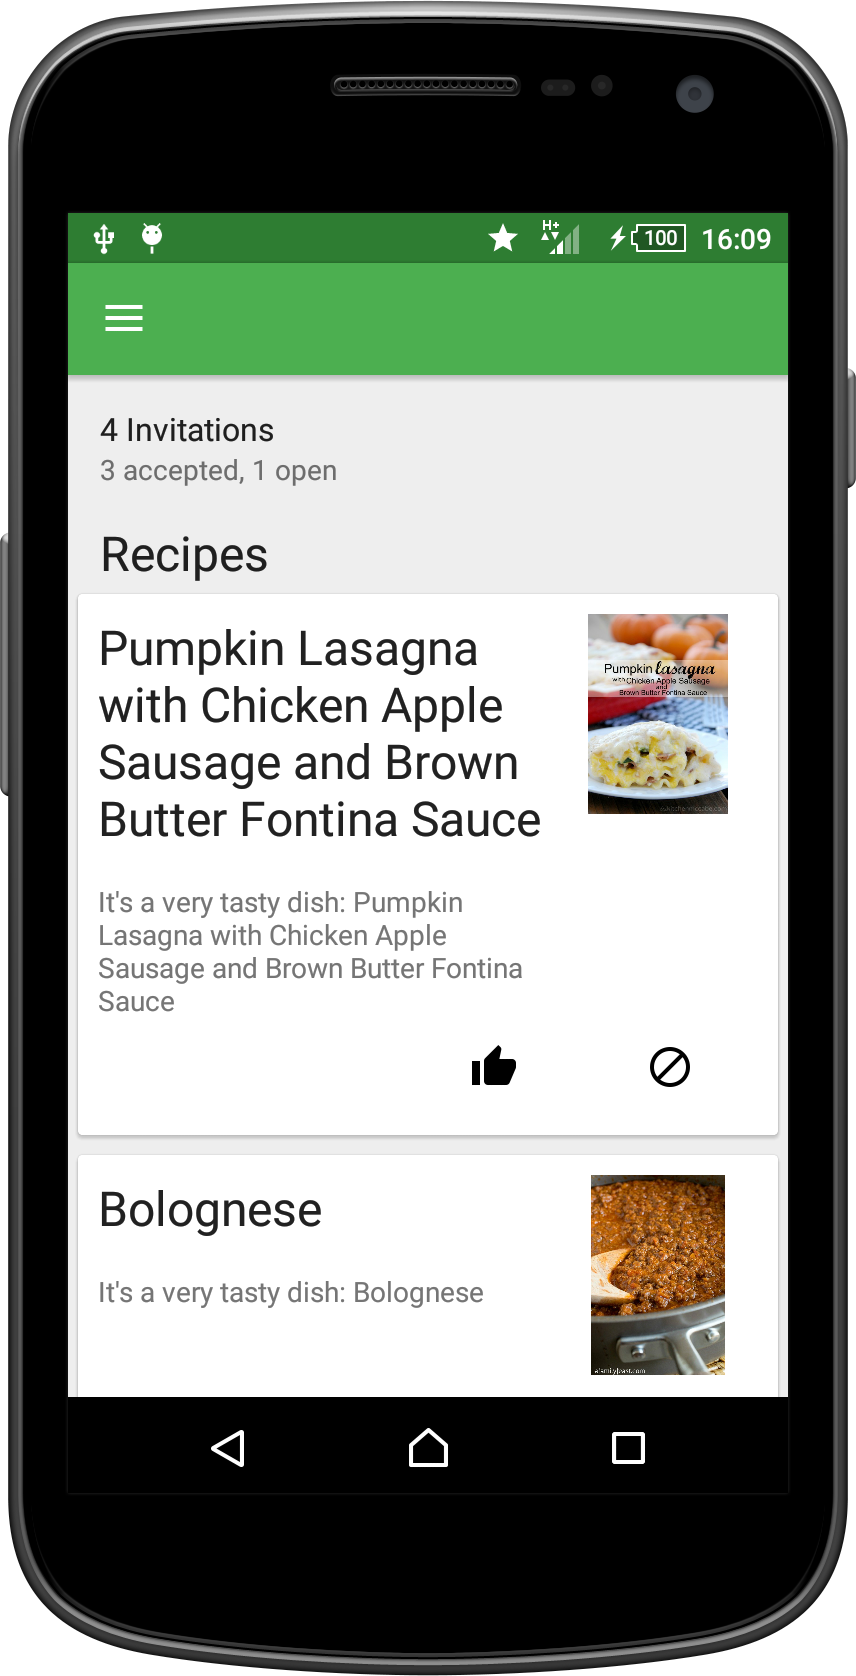
\includegraphics[width=0.2\textwidth,height=\textheight,keepaspectratio]{../screenshots/recipe_overview.png}
                \hspace{0.2cm}
                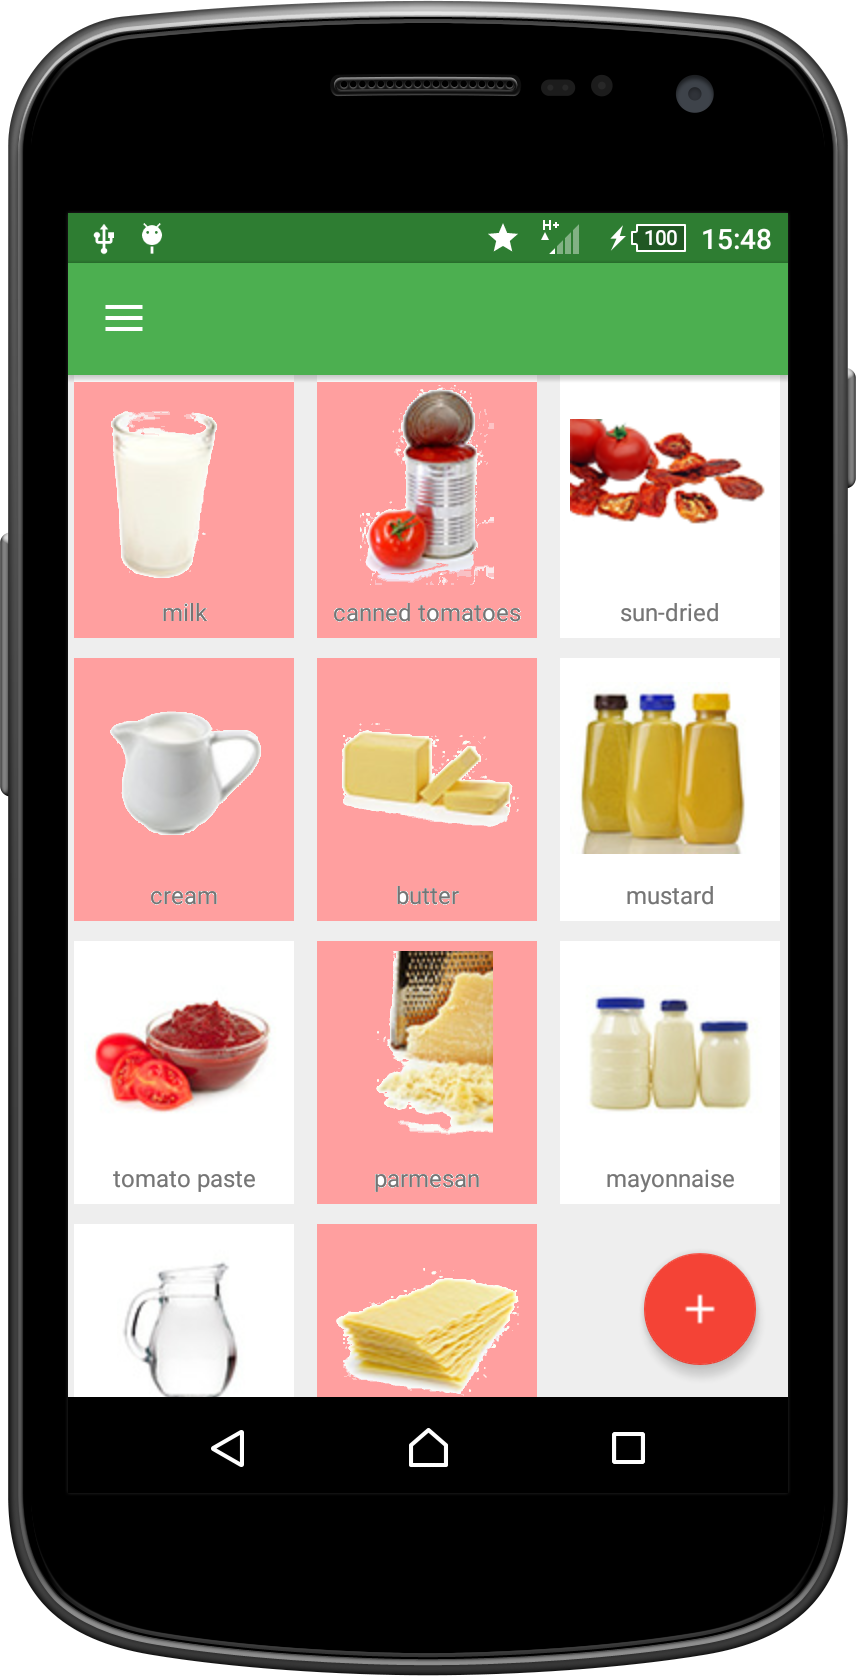
\includegraphics[width=0.2\textwidth,height=\textheight,keepaspectratio]{../screenshots/recipe_ingredients.png}
                \hspace{0.5cm}
                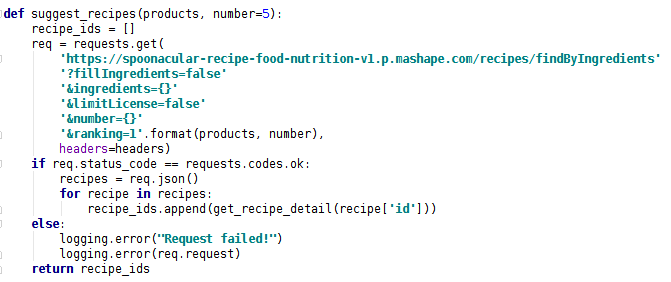
\includegraphics[width=0.5\textwidth,height=\textheight,keepaspectratio]{../screenshots/suggest_recipes_api_servercode.png}
            \end{center}
        \end{figure}
    }

    \frame{\frametitle{Location adaptation}
        \begin{itemize}
            \item Find groups of people nearby
            \item Server calculates groups by location
            \item Technology used: PostgreSQL Database with PostGIS Extension for location features
            \begin{itemize}
                \item PostGIS function example used in SQL Query: $ST\_DISTANCE(user1.location, user2.location) \textless $1500
                \item Returns TRUE if user1 is in a 1.5km range of user2
            \end{itemize}
            \item Example: user\_id has X possible group\_members in a range of max\_distance
        \end{itemize}
        \begin{figure}
            \begin{center}
                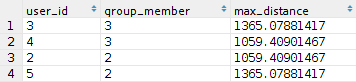
\includegraphics[width=0.4\textwidth,height=\textheight,keepaspectratio]{../screenshots/group_sql.png}
            \end{center}
        \end{figure}
    }

\section{Adaptation on Technical Context}
  \frame{\frametitle{Adaptation of Communication}
        \begin{itemize}
          \item ``Adapt the way data is exchanged between distributed components''
          \item A ConnectivityManager checks if a NetworkConnection is availiable:
          \begin{itemize}
            \item If there is one the Call gets executed
            \item On Error or with no Connection the Calls are persisted
          \end{itemize}
        %  \item API Calls are cached or persisted, until network is available
          \item We use com.birbit.android.jobqueue for queueing API Calls
        \end{itemize}
        \begin{figure}
          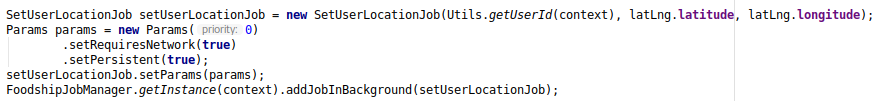
\includegraphics[width=0.8\textwidth,height=\textheight,keepaspectratio]{../screenshots/jobqueue_example.png}
        \end{figure}
    }

    \frame{\frametitle{Adaptation of Connectivity}
        \begin{itemize}
          \item Push notification triggered by our server
          \item App then prefetches group information and recipe pictures
          \item Data is persisted in internal storage and in cache for better user experience
        \end{itemize}
        \begin{figure}
          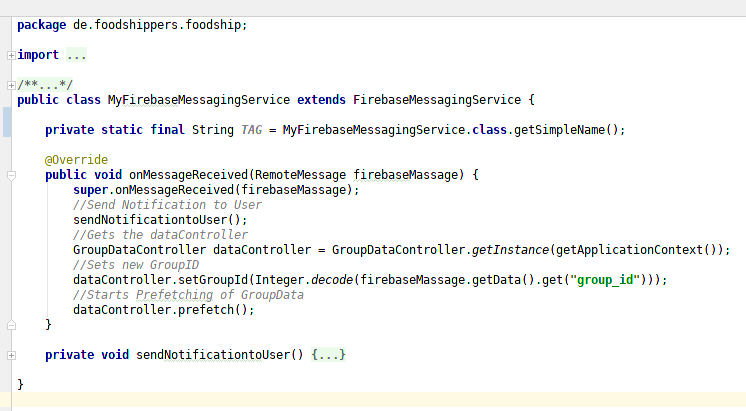
\includegraphics[width=0.8\textwidth,height=\textheight,keepaspectratio]{../screenshots/prefetching.png}
        \end{figure}
    }

\section{Architecture}
    \frame{\frametitle{Architecture \& Technologies}
        \begin{figure}
          \centering
          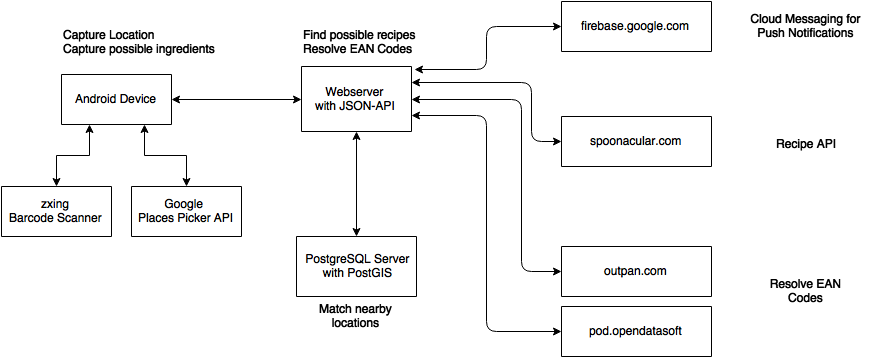
\includegraphics[width=0.9\textwidth,height=\textheight,keepaspectratio]{../diagrams/architecture_2.png}
        \end{figure}
    }
\section{Work}
  \frame{\frametitle{Whats next?}
    \begin{itemize}
      \item Better integration of the dinner groups into the app
      \item Image size adaptation depending on the network speed
      \item Testing with more devices in real environment
      \item Final Presentation
    \end{itemize}
  }

\end{document}
